\documentclass[10pt]{article}
\newcommand{\doctitle}{GraphRAG Project Proposal}
% Shared layout for the CTRL ALT DEFEAT documents (compile with xelatex).
\usepackage{fontspec}
\setmainfont{TeX Gyre Termes}
\setsansfont{TeX Gyre Heros}
\setmonofont{DejaVu Sans Mono}[Scale=0.80]
\usepackage[letterpaper, top=0.72in, bottom=0.78in, left=0.8in, right=0.8in,
            headheight=13pt, headsep=9pt, footskip=22pt]{geometry}
\usepackage{microtype}
\linespread{1.02}
\usepackage{xcolor}
\definecolor{ink}{HTML}{1F2A44}
\definecolor{accent}{HTML}{3B5B92}
\definecolor{attc}{HTML}{3B5B92}
\definecolor{attf}{HTML}{E8EFF9}
\definecolor{txtc}{HTML}{B5651D}
\definecolor{txtf}{HTML}{FDF0E2}
\definecolor{evalc}{HTML}{3C7A50}
\definecolor{evalf}{HTML}{E6F3EA}
\definecolor{rulec}{HTML}{C9D3E3}
\definecolor{shade}{HTML}{F4F7FB}
\usepackage{titlesec}
\titleformat{\section}{\sffamily\bfseries\large\color{ink}}{\thesection}{0.55em}{}
\titlespacing*{\section}{0pt}{8pt}{2pt}
\titleformat{\subsection}[runin]{\sffamily\bfseries\normalsize\color{ink}}{\thesubsection}{0.45em}{}[.]
\titlespacing*{\subsection}{0pt}{4pt}{0.55em}
\usepackage{enumitem}
\setlist{nosep, leftmargin=1.15em, topsep=1pt, itemsep=1pt}
\usepackage{booktabs, tabularx, array, multirow, makecell}
\renewcommand{\arraystretch}{1.12}
\newcolumntype{L}{>{\raggedright\arraybackslash}X}
\newcolumntype{P}[1]{>{\raggedright\arraybackslash}p{#1}}
\usepackage{graphicx}
\usepackage{caption}
\captionsetup{font={small,sf}, labelfont={bf,color=ink}, skip=3pt}
\usepackage{float}
\usepackage{tikz}
\usetikzlibrary{arrows.meta, positioning, calc, fit, backgrounds}
\usepackage{listings}
\lstset{basicstyle=\ttfamily\scriptsize, columns=fullflexible, keepspaces=true, breaklines=true,
        frame=single, rulecolor=\color{rulec}, backgroundcolor=\color{shade}, framesep=3pt,
        xleftmargin=3pt, xrightmargin=3pt, aboveskip=3pt, belowskip=3pt, showstringspaces=false,
        breakatwhitespace=true, upquote=true}
\usepackage{fancyhdr, lastpage}
\pagestyle{fancy}
\fancyhf{}
\renewcommand{\headrulewidth}{0.4pt}
\fancyhead[L]{\sffamily\footnotesize\color{ink}CTRL ALT DEFEAT \textbullet\ \doctitle}
\fancyhead[R]{\sffamily\footnotesize\color{ink}CS 6338 Knowledge Engineering}
\fancyfoot[C]{\sffamily\footnotesize\color{ink}Page \thepage\ of \pageref{LastPage}}
\fancypagestyle{first}{\fancyhf{}\renewcommand{\headrulewidth}{0pt}%
  \fancyfoot[C]{\sffamily\footnotesize\color{ink}Page \thepage\ of \pageref{LastPage}}}
\usepackage[hidelinks]{hyperref}
\setlength{\parindent}{0pt}
\setlength{\parskip}{3pt}
\newcommand{\code}[1]{\texttt{#1}}
\renewcommand{\cite}[1]{[#1]}
% A small rounded label for the subsystem numbers in the figures
\newcommand{\badge}[1]{\tikz[baseline=(b.base)]\node[circle, fill=ink, text=white, inner sep=1pt,
  minimum size=9pt, font=\sffamily\bfseries\tiny](b){#1};}
\tikzset{
  box/.style={draw, rounded corners=2.5pt, align=center, inner sep=3pt, font=\sffamily\scriptsize, line width=0.6pt,
    execute at begin node={\hyphenpenalty=10000\exhyphenpenalty=10000\relax}},
  txtbox/.style={box, draw=txtc, fill=txtf},
  attbox/.style={box, draw=attc, fill=attf},
  evalbox/.style={box, draw=evalc, fill=evalf},
  plainbox/.style={box, draw=ink!60, fill=white},
  flow/.style={-{Stealth[length=4pt, width=3.4pt]}, line width=0.6pt, draw=ink!75},
  rel/.style={-{Stealth[length=4pt, width=3.4pt]}, line width=0.6pt},
  lab/.style={font=\sffamily\tiny, fill=white, inner sep=0.8pt},
}

\hypersetup{pdftitle={CTRL ALT DEFEAT: GraphRAG Project Proposal}, pdfauthor={Shane Waldrop}}
\usepackage{multicol}
\renewcommand{\badge}[1]{\tikz[baseline=(b.base)]\node[circle, fill=ink, text=white, inner sep=0.6pt, minimum size=10.5pt, font=\sffamily\bfseries\scriptsize](b){#1};}
\newcommand{\figcode}{\renewcommand{\code}[1]{\textsf{##1}}}

\begin{document}
\thispagestyle{first}

{\sffamily
{\color{accent}\footnotesize\bfseries CS 6338 KNOWLEDGE ENGINEERING \textbullet\ TERM PROJECT PROPOSAL (MILESTONE 1)}\par\vspace{2pt}
{\color{ink}\LARGE\bfseries Intelligent GraphRAG Chatbot for Cyber Threat Reports}\par\vspace{3pt}
{\small Team \textbf{CTRL ALT DEFEAT} \textbullet\ Shane Waldrop (swaldrop2@angelo.edu)\\ Angelo State University \textbullet\ Instructor: Dr.\ Erdogan Dogdu \textbullet\ October 2026}\par}
\vspace{4pt}
\noindent\colorbox{shade}{\parbox{\dimexpr\textwidth-2\fboxsep}{\small
\textbf{Summary.} The system answers a threat analyst's multi-hop questions about cyber threat reports, meaning questions whose answers join several linked facts. It is a GraphRAG system (graph retrieval-augmented generation): a Neo4j knowledge graph joins the AnnoCTR reports with MITRE ATT\&CK (Adversarial Tactics, Techniques, and Common Knowledge) version 20.0, the structured catalogue of adversary behaviour. A large language model (LLM) extracts from each report the ATT\&CK techniques, tactics, groups and software it names or describes. Answers come from retrieved report text plus the graph around the entities in it; the model is told to cite the report chunk or graph relationship behind every statement, and code checks that each cited ID was in its context. \textbf{Status on 19 October 2026:} the pipeline runs end to end on one development report, and the benchmark (682 gold triples, 24 multi-hop questions) is built and verified.}}

\section{Team \& Role Distribution}
Team name: \textbf{CTRL ALT DEFEAT}. Member: Shane Waldrop, swaldrop2@angelo.edu. The course specifies teams of two to three students; this team has one member, who holds every role in Table~\ref{tab:roles}, so the secondary column reads ``none''. The checks a second member would provide are automated instead: 86 automated tests, a recomputation of every benchmark answer by Cypher (Neo4j's query language) inside Neo4j, and an independent reimplementation of the benchmark (Section~\ref{sec:data}).

\begin{table}[H]\centering\small
\caption{Component ownership matrix (UI: user interface).}\label{tab:roles}
\begin{tabularx}{\textwidth}{@{}P{3.9cm}LP{2.1cm}P{1.5cm}@{}}
\toprule
Role & Responsibilities in this project & Primary & Secondary\\
\midrule
Data \& Annotation Lead & AnnoCTR and ATT\&CK data audit; gold triples; question set; verification & S.\ Waldrop & none\\
Graph Extraction \& Reasoning Lead & extraction prompt, checks; linking to ATT\&CK; RDF/OWL ontology (Resource Description Framework / Web Ontology Language); fusion, inference rule; GDS (Neo4j Graph Data Science) analytics & S.\ Waldrop & none\\
Embedding \& Retrieval Lead & chunk and graph embeddings; vector indexes; personalized-PageRank retrieval & S.\ Waldrop & none\\
Evaluation \& UI Lead & scorer; RAGAS (Retrieval-Augmented Generation Assessment) metrics; blind rating sheet and rating; Streamlit chat page & S.\ Waldrop & none\\
\bottomrule
\end{tabularx}
\end{table}

\section{Problem Statement \& Domain Context}
\textbf{Domain.} Cyber threat intelligence (CTI). Security vendors publish threat reports in prose; analysts translate them into MITRE ATT\&CK \cite{2}, the public catalogue of adversary behaviour (v20.0, released 13 October 2026: 15 tactics, 706 techniques of which 479 are sub-techniques, 178 groups, 842 software, 44 mitigations), to decide which detections and mitigations matter.

\textbf{Why text-only RAG struggles here.} Retrieval-augmented generation (RAG) hands the $k$ report chunks most similar to the question to a language model \cite{3}. It struggles with four kinds of question analysts ask:
\begin{enumerate}[label=(\arabic*), leftmargin=*]
\item \emph{The answer is not in the report.} Mitigations, a group's known software and a technique's tactics are ATT\&CK facts that reports rarely state. Measured on the \emph{tracer report}, a development (dev) report run end to end as the first test (Lab52, June 2020, Mustang Panda): asked which ATT\&CK mitigations address the report's techniques, the text-only baseline replied that its context names no mitigations, while the graph-enriched pipeline named four (M1038, M1047, M1017, M1031) with 10 citations, each pointing to a fact in its context. The four follow the system's own links, which missed five of the eight expert-labelled techniques, among them T1036 and T1055; M1022 and M1040, which address the most expert-labelled techniques, are absent. Section~\ref{sec:eval} measures answer quality.
\item \emph{Behaviour is described, not named.} Of the 1,526 expert links to ATT\&CK in the test reports, 691 (45\%) are implicit (in a dev report, ``with a legitimate binary'' is linked to T1036 Masquerading), and only 288 mention texts (19\%) equal an ATT\&CK name or alias, compared ignoring case.
\item \emph{Questions chain and aggregate facts.} ``Which mitigation addresses the most techniques in report $R$?'' needs every technique of $R$, every MITIGATES relationship into those techniques (27 to 192 for the five such benchmark questions) and a count. Similarity search over chunks supplies none of those joins; the graph supplies them, and the planned engine computes the counts in Cypher before the model answers (Section~\ref{sec:arch}(d)).
\item \emph{The catalogue moves.} Recent ATT\&CK releases renamed the tactic Defense Evasion to Stealth, added Defense Impairment and revoked T1562 in favour of T1685. A model's memory of older releases gives outdated names; a graph loaded from v20.0 carries the current ones.
\end{enumerate}
\textbf{Persona.} A security operations center (SOC) or CTI analyst who reads vendor reports, must prioritise defences, and needs each claim traceable to the report sentence or ATT\&CK relationship behind it.
\textbf{Questions the chatbot answers.} Ten multi-hop patterns (Table~\ref{tab:patterns}); each benchmark question names its report $R$ by vendor, month and title.

\begin{table}[H]\centering\small
\caption{The ten question patterns, with the number of benchmark questions ($n$) of each.}\label{tab:patterns}
\begin{tabularx}{\textwidth}{@{}Lp{0.35cm}Lp{0.35cm}@{}}
\toprule
Pattern & $n$ & Pattern & $n$\\
\midrule
Mitigations that address the most of $R$'s techniques & 5 & $R$'s techniques that ATT\&CK records group $G$ as using & 2\\
Tactics under which ATT\&CK places $R$'s techniques & 4 & Group in $R$ that uses the most of $R$'s techniques & 1\\
Software in $R$ that the group in $R$ uses & 2 & $R$'s techniques that ATT\&CK records software $S$ as using & 3\\
Groups in $R$ that use the software in $R$ & 1 & $R$'s techniques missing from ATT\&CK's record of $S$ & 1\\
Groups that use every technique of $R$ & 2 & Techniques that reports $R_1$ and $R_2$ both describe & 3\\
\bottomrule
\end{tabularx}
\end{table}

\section{Dataset \& Ground-Truth Verification Plan}\label{sec:data}
\textbf{Text corpus.} AnnoCTR \cite{1}: the 120 English threat reports (2016--2022) that carry AnnoCTR's cybersecurity annotation layer, donated by Intel 471, Lab52 (S2 Grupo), Proofpoint, QuoIntelligence and Zscaler; 1.20 million characters (152,887 words) after embedded images are removed; split by its authors into 70 train, 16 dev and 34 test reports; licence CC BY-SA 4.0 (source commit \code{d510b69}). \textbf{Structured source.} MITRE ATT\&CK v20.0 Enterprise, a STIX (Structured Threat Information Expression) 2.0 JSON (JavaScript Object Notation) bundle of 49\,MB: 1,785 live entries and 19,545 relationship objects are used, plus 881 technique-to-tactic links read from the techniques' kill-chain phases (20,426 relationships in all).

\textbf{Existing annotations.} Domain experts marked mentions of techniques, tactics, groups and software and linked them to ATT\&CK: 5,626 links (train 3,326, dev 774, test 1,526). AnnoCTR has no expert labels for relations between entities, so the ``uses'' relations the model extracts cannot be scored against expert labels.

\textbf{Gold triples (minimum 50; built 682).} One triple (report, \code{MENTIONS}, ATT\&CK entry) for every entry the experts linked in all 16 dev and 34 test reports; in the graph, a triple stands for the path Report\,$\rightarrow$\,HAS\_CHUNK\,$\rightarrow$\,Chunk\,$\rightarrow$\,MENTIONS\,$\rightarrow$\,entry. The triples cover those reports completely, not a sample, so precision is measurable against the experts' labels, though a correct link they did not make counts as an error (the tracer report has one, APT27 $\rightarrow$ G0027), and a second annotator's technique sets agree with the first at only 54\% average F1 (the harmonic mean of precision and recall) \cite{1}. Expert IDs are mapped to v20.0: 10 report-level links to the revoked T1562 become T1685, and 6 report-level links (10 mentions) to ATT\&CK Mobile IDs, absent from the Enterprise domain, are set aside. Test: 469 triples (327 techniques, 85 tactics, 13 groups, 44 software); dev: 213. Every technique label names a parent technique, never a sub-technique.

\textbf{Multi-hop question--answer (QA) pairs (minimum 20; built 24).} Pairs in ten patterns over 20 of the 34 test reports, chosen from the gold facts and never from system output, with answers of 1 to 6 items. Each answer is computed from the gold triples and ATT\&CK, never from the system's own graph, and each question stores a reference answer in words, its supporting facts and a Cypher query. Because the experts label parent techniques, a relationship that ATT\&CK records for a sub-technique counts for its parent.

\textbf{Verification.} (i) Both files are written by a committed script, \code{gold.py}; a test rebuilds them and fails on any difference. (ii) Each question's Cypher query recomputes its answer inside Neo4j: 24 of 24 agree (measured 19 October). (iii) A separate reimplementation from the raw files reproduced all 24 answers and the test gold totals. (iv) Three answers were compared item by item with attack.mitre.org pages, read through an automated page reader.
\textbf{Split discipline.} Train reports supply the prompt's two worked examples only; dev reports are for trying changes and calibrating the linking threshold; the test reports run once, for the reported numbers.

\section{Target Knowledge Graph Schema \& Ontology}
\begin{figure}[tb]\centering
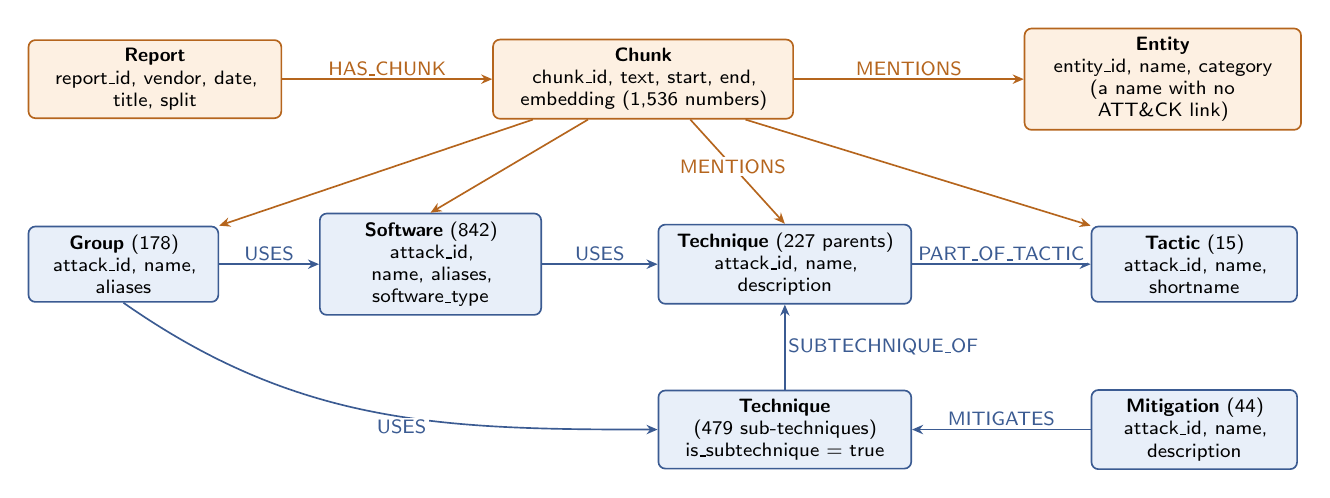
\begin{tikzpicture}[x=1cm, y=1cm]
\tikzset{elab/.style={font=\sffamily\scriptsize, fill=white, inner sep=1pt}}
\node[txtbox, text width=3.0cm] (report) at (1.7,2.35) {\textbf{Report}\\report\_id, vendor, date,\\title, split};
\node[txtbox, text width=3.6cm] (chunk) at (7.9,2.35) {\textbf{Chunk}\\chunk\_id, text, start, end,\\embedding (1,536 numbers)};
\node[txtbox, text width=3.3cm] (entity) at (14.5,2.35) {\textbf{Entity}\\entity\_id, name, category\\(a name with no ATT\&CK link)};
\node[attbox, text width=2.2cm] (group) at (1.3,0) {\textbf{Group} (178)\\attack\_id, name,\\aliases};
\node[attbox, text width=2.6cm] (software) at (5.2,0) {\textbf{Software} (842)\\attack\_id, name, aliases,\\software\_type};
\node[attbox, text width=3.0cm] (technique) at (9.7,0) {\textbf{Technique} (227 parents)\\attack\_id, name,\\description};
\node[attbox, text width=2.4cm] (tactic) at (14.9,0) {\textbf{Tactic} (15)\\attack\_id, name,\\shortname};
\node[attbox, text width=3.0cm] (sub) at (9.7,-2.1) {\textbf{Technique}\\(479 sub-techniques)\\is\_subtechnique = true};
\node[attbox, text width=2.4cm] (mitigation) at (14.9,-2.1) {\textbf{Mitigation} (44)\\attack\_id, name,\\description};
\draw[rel, txtc] (report) -- node[elab, above, text=txtc]{HAS\_CHUNK} (chunk);
\draw[rel, txtc] (chunk) -- node[elab, above, text=txtc]{MENTIONS} (entity);
\draw[rel, txtc] ($(chunk.south)+(-1.4,0)$) -- (group.north east);
\draw[rel, txtc] ($(chunk.south)+(-0.7,0)$) -- (software.north);
\draw[rel, txtc] ($(chunk.south)+(0.6,0)$) -- node[elab, text=txtc, pos=0.45]{MENTIONS} (technique.north);
\draw[rel, txtc] ($(chunk.south)+(1.3,0)$) -- (tactic.north west);
\draw[rel, attc] (group) -- node[elab, above, text=attc]{USES} (software);
\draw[rel, attc] (software) -- node[elab, above, text=attc]{USES} (technique);
\draw[rel, attc] (group.south) to[out=-35, in=180] node[elab, below, text=attc, pos=0.55]{USES} (sub.west);
\draw[rel, attc] (technique) -- node[elab, above, text=attc]{PART\_OF\_TACTIC} (tactic);
\draw[rel, attc] (sub) -- node[elab, right, text=attc]{SUBTECHNIQUE\_OF} (technique);
\draw[rel, attc] (mitigation) -- node[elab, above, text=attc]{MITIGATES} (sub);
\end{tikzpicture}
\caption{Knowledge-graph schema. Orange: nodes and relationships from reports (\code{source = "text"}); blue: MITRE ATT\&CK v20.0 (\code{source = "attack"}) with live entry counts. Sub-techniques are Technique nodes. MENTIONS reaches any ATT\&CK node, sub-techniques and mitigations included, or an Entity; USES and MITIGATES reach techniques and sub-techniques alike.}\label{fig:schema}
\end{figure}
\textbf{Node types.} Report; Chunk (a 4,000-character window); the five ATT\&CK classes Technique (including sub-techniques), Tactic, Group, Software and Mitigation; Entity (a name the linker could not tie to ATT\&CK).
\textbf{Relationship types.} \code{HAS\_CHUNK}; \code{MENTIONS} (chunk to the entry it names or describes); \code{USES} (from ATT\&CK: group to technique, software to technique, group to software; from text, between whatever entries or Entity nodes the two mentions link to); \code{SUBTECHNIQUE\_OF}; \code{PART\_OF\_TACTIC}; \code{MITIGATES}.
\textbf{Key attributes.} Every relationship carries \code{edge\_id} (the ID that answers cite) and \code{source} (\code{attack} or \code{text}). \code{MENTIONS} adds \code{report\_id}, \code{chunk\_id}, the mention text, the verbatim evidence sentence, \code{link\_method}, \code{confidence} (1.0 for an exact name match, the cosine similarity for an embedding match), the model's own confidence (stored; the dev calibration tests a cut-off on it), the model name and the extraction timestamp. One uniqueness constraint per node label guards every key.
\textbf{Ontology.} ATT\&CK enters as RDF/OWL built with rdflib: OWL classes for the five ATT\&CK kinds and object properties \code{uses}, \code{mitigates}, \code{subtechniqueOf} and \code{partOfTactic} (194,611 triples). RDF 1.1 cannot attach properties to a triple, so each relationship is also an \code{rdf:Statement} carrying its \code{edgeId}, \code{source} and description; Neo4j's labeled property graph (LPG) stores the same properties on the relationship itself.

\section{Proposed GraphRAG System Architecture}\label{sec:arch}
\begin{figure}[tb]\centering\figcode
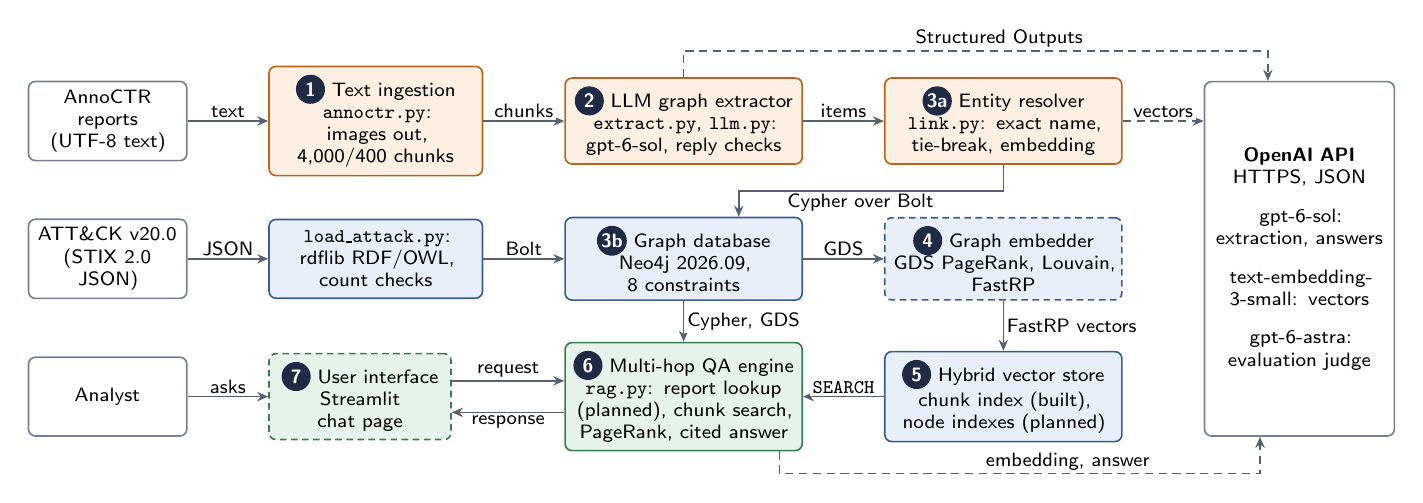
\begin{tikzpicture}[x=1cm, y=1cm]
\tikzset{c1/.style={text width=1.8cm, minimum height=1.0cm}, c2/.style={text width=2.5cm, minimum height=1.0cm},
  c3/.style={text width=2.8cm, minimum height=1.0cm}, planned/.style={dash pattern=on 2.4pt off 1.6pt},
  elab/.style={font=\sffamily\scriptsize, fill=white, inner sep=1pt}, call/.style={flow, dash pattern=on 3pt off 2pt}}
\node[plainbox, c1] (src) at (1.01,0) {AnnoCTR reports\\(UTF-8 text)};
\node[txtbox, c2] (ing) at (4.415,0) {\badge{1} Text ingestion\\\code{annoctr.py}: images out,\\4,000/400 chunks};
\node[txtbox, c3] (ext) at (8.325,0) {\badge{2} LLM graph extractor\\\code{extract.py}, \code{llm.py}:\\gpt-6-sol, reply checks};
\node[txtbox, c3] (ned) at (12.385,0) {\badge{3a} Entity resolver\\\code{link.py}: exact name,\\tie-break, embedding};
\node[plainbox, text width=2.2cm, minimum height=4.5cm] (oai) at (16.145,-1.75) {\textbf{OpenAI API}\\HTTPS, JSON\\[6pt]gpt-6-sol:\\extraction, answers\\[6pt]text-embedding-\\3-small: vectors\\[6pt]gpt-6-astra:\\evaluation judge};
\node[plainbox, c1] (stix) at (1.01,-1.75) {ATT\&CK v20.0\\(STIX 2.0 JSON)};
\node[attbox, c2] (rdf) at (4.415,-1.75) {\code{load\_attack.py}:\\rdflib RDF/OWL,\\count checks};
\node[attbox, c3] (neo) at (8.325,-1.75) {\badge{3b} Graph database\\Neo4j 2026.09,\\8 constraints};
\node[attbox, c3, planned] (emb) at (12.385,-1.75) {\badge{4} Graph embedder\\GDS PageRank, Louvain,\\FastRP};
\node[plainbox, c1] (an) at (1.01,-3.5) {Analyst};
\node[evalbox, text width=2.1cm, minimum height=1.0cm, planned] (ui) at (4.215,-3.5) {\badge{7} User interface\\Streamlit chat page};
\node[evalbox, c3] (qa) at (8.325,-3.5) {\badge{6} Multi-hop QA engine\\\code{rag.py}: report lookup\\(planned), chunk search,\\PageRank, cited answer};
\node[attbox, c3] (vec) at (12.385,-3.5) {\badge{5} Hybrid vector store\\chunk index (built),\\node indexes (planned)};
\draw[flow] (src) -- node[elab, above]{text} (ing);
\draw[flow] (ing) -- node[elab, above]{chunks} (ext);
\draw[flow] (ext) -- node[elab, above]{items} (ned);
\draw[flow] (stix) -- node[elab, above]{JSON} (rdf);
\draw[flow] (rdf) -- node[elab, above]{Bolt} (neo);
\draw[flow] (neo) -- node[elab, above]{GDS} (emb);
\draw[flow] (ned.south) -- ++(0,-0.33) -| node[elab, pos=0.27, below]{Cypher over Bolt} ($(neo.north)+(0.7,0)$);
\draw[flow] (emb.south) -- node[elab, right]{FastRP vectors} (vec.north);
\draw[flow] (vec) -- node[elab, above]{\code{SEARCH}} (qa);
\draw[flow] (neo.south) -- node[elab, right]{Cypher, GDS} (qa.north);
\draw[flow] (an) -- node[elab, above]{asks} (ui);
\draw[flow] ($(ui.east)+(0,0.2)$) -- node[elab, above]{request} ($(qa.west)+(0,0.2)$);
\draw[flow] ($(qa.west)+(0,-0.2)$) -- node[elab, below]{response} ($(ui.east)+(0,-0.2)$);
\draw[call] (ext.north) -- ++(0,0.33) -| node[elab, pos=0.27, above]{Structured Outputs} ($(oai.north)+(-0.4,0)$);
\draw[call] (ned) -- node[elab, above]{vectors} (ned -| oai.west);
\draw[call] ($(qa.south east)+(-0.3,0)$) -- ++(0,-0.28) -| node[elab, pos=0.3, above]{embedding, answer} ($(oai.south)+(-0.5,0)$);
\end{tikzpicture}
\caption{Architecture: the seven subsystems of the design (1 text ingestion, 2 LLM graph extractor, 3a entity resolver and 3b graph database, 4 graph embedder, 5 hybrid vector store, 6 multi-hop question-answering (QA) engine, 7 user interface). Dashed outline: not built yet. Dashed arrow: an HTTPS (encrypted web) call to the OpenAI application programming interface (API). Neo4j holds the graph and every vector index. FastRP: fast random projection.}\label{fig:arch}
\end{figure}

\subsection*{(a) LLM extraction} gpt-6-sol (OpenAI) at reasoning effort \emph{none}, temperature 0 and seed 7, at most 4,000 output tokens per call. Replies are forced into a JSON schema generated from Pydantic models: mentions (id, text, category, ATT\&CK name, evidence sentence, confidence) and ``uses'' relations between mention ids. Two worked examples from train reports precede each chunk. Chunks hold 4,000 characters with a 400-character overlap (dev 50, test 99 chunks). Code, not the model, assigns every permanent ID and checks each item against the chunk text; 13 reasons for dropping output are counted separately (tracer report, 19 October, earlier one-example prompt, the run behind every tracer figure here: 29 mentions and 9 relations kept, none dropped). Every reply is saved under a hash of its request, so reruns are identical and free. A local model (qwen3:4b, run with Ollama) will be shown on one chunk.

\subsection*{(b) Graph enhancement \& verification} \emph{Entity resolution} (named entity disambiguation) links each mention to ATT\&CK: exact match of the model's ATT\&CK name, then of the mention text, against 2,927 keys (2,448 distinct names and aliases, compared ignoring case and punctuation, plus 479 ``Parent: Sub-technique'' names) across all five ATT\&CK kinds; written tie-break rules for the 49 keys shared by several entries; otherwise embedding similarity (text-embedding-3-small over each entry's name and description) above a threshold to be calibrated on the 213 dev facts (provisionally cosine 0.40); otherwise an Entity node keyed by category and normalised name, so repeated unlinked names merge (measured on the tracer report: 23 exact and 6 embedding links). \emph{Reasoning} has two layers: data fusion of ATT\&CK, the external structured source, with the extracted report facts; and an inference rule, applied in every benchmark query, that a relationship ATT\&CK records for a sub-technique also holds for its parent technique. GDS adds PageRank, Louvain communities \cite{8} and FastRP (fast random projection) embeddings in the full build (Phase 5), for the final report's analysis and the chat page's ``similar entries''; they stay out of the answer prompt, because a similarity score is not a citable fact. \emph{Verification}: \code{score.py} compares the system's facts with the gold triples (Section~\ref{sec:eval}).

\subsection*{(c) Embedding \& indexing} Chunk embeddings come from text-embedding-3-small (1,536 numbers) in a Neo4j vector index: HNSW (hierarchical navigable small world) \cite{9}, cosine similarity, no quantization. Graph embeddings will come from FastRP \cite{7}: 128 dimensions, fixed random seed, one thread, over the ATT\&CK graph, stored in vector indexes for Technique, Group and Software. Louvain community IDs and PageRank scores will become node properties. Analytics outputs will be saved to files and reloaded, so every machine uses the same values. Neo4j serves as both graph store and vector store.

\subsection*{(d) Retrieval \& generation} The engine will first look up (planned) the report a question names, matching a quoted title against the Report nodes' titles, and takes the 4 chunks most similar to the question (planned: from that report when one is found). The entities those chunks mention (planned: and every entity the named report mentions), ATT\&CK entries and Entity nodes alike, seed a personalized PageRank \cite{6} over ATT\&CK's relationships and the ``uses'' relations found in text, the retrieval idea of HippoRAG \cite{5}; Microsoft's GraphRAG \cite{4} instead summarises communities of an LLM-built graph for corpus-wide questions. Among the 200 best-scoring nodes, summary lines (planned) state for each nearby ATT\&CK entry how many of the report's entities it links to, with an edge ID per link, so a counting question gets counts computed in Cypher. Then come up to 40 mention facts and at most 60 relationship facts (seed to seed first, then one step out, then two, taken in turn from each type). The prompt template tells the model to use only that context and to cite after every statement, as \code{[chunk:ID]} or \code{[edge:ID]}; code then checks that every cited ID was in the context. A Streamlit page will show the answer, its citations, and the chunks and facts used.

\section{Evaluation \& Benchmarking Strategy}\label{sec:eval}
\textbf{Automated metrics.}
\begin{itemize}
\item \emph{Entity extraction and linking:} precision, recall and F1 of (report, ATT\&CK entry) facts against the 469 test gold triples, overall and per kind, at sub-technique and parent level, with a scorer tested on five hand-made cases. Reported beside a baseline that links every ATT\&CK name or alias found verbatim (ignoring case) in a report's text, and, for context, the AnnoCTR paper's best document-level F1 (techniques 56.6, tactics 47.7, sub-techniques collapsed to parents). Measured on the tracer report: F1 0.519 at sub-technique level, 0.593 at parent level.
\item \emph{Answer accuracy:} per question, precision, recall and F1 of the IDs of the kind the question asks for, named in the answer outside its citations, against the answer IDs stored with each question, averaged over the 24 questions.
\item \emph{RAGAS} \cite{10}: faithfulness, answer relevance and context recall, judged by gpt-6-astra. Language-model judges can favour text that resembles their own output \cite{11,12,13}, and the answer model and the judge are both OpenAI GPT-6 models, so RAGAS scores are reported as a judge's estimate, with one judge for both systems, beside the human ratings.
\item \emph{Operations:} citation-ID validity rate, latency per stage, cost per question.
\end{itemize}
\textbf{Human testing.} Both systems answer all 24 questions. Before rating, a script replaces each citation with a neutral number and lists the cited texts in one format for both systems (raw citations would reveal the system, since only GraphRAG cites graph facts), then shuffles each question's two answers with a fixed seed and labels them A and B. The rater scores the 48 answers from 1 to 5 on Factuality, Completeness and Coherence against the anchors in Table~\ref{tab:rubric} and the reference answers. The rater is the member who built the system, and the kind of evidence cited can still hint at the system; the ID-based answer accuracy needs no rater.
\textbf{Baseline.} The same pipeline with the graph switched off: same question embedding, same 4 chunks, same model and citation rules, no graph facts.

\begin{table}[tb]\centering\small
\caption{Human rating anchors (2 and 4 lie between the neighbouring anchors). Completeness follows the share of the reference answer's items given, so a one-item answer scores 5 or 1.}\label{tab:rubric}
\begin{tabularx}{\textwidth}{@{}p{0.9cm}LLL@{}}
\toprule
Score & Factuality & Completeness & Coherence\\
\midrule
5 & every statement correct and supported by its citation & every item of the reference answer & direct, well organised, no repetition\\
3 & mostly correct; one material error & at least half of the items & understandable, some disorder\\
1 & mostly wrong or unsupported & none of the items & incoherent or off the question\\
\bottomrule
\end{tabularx}
\end{table}

\section{Technical Risk Analysis \& Mitigation Plan}
Table~\ref{tab:risks} lists the six main technical risks, each with its mitigation and the evidence so far.
\begin{table}[tb]\centering\small
\caption{Main technical risks.}\label{tab:risks}
\begin{tabularx}{\textwidth}{@{}P{4.1cm}L@{}}
\toprule
Risk & Mitigation (and evidence so far)\\
\midrule
API cost and rate limits & Every reply saved and reused: the tracer run cost about \$0.07 (measured tokens at list prices); all 149 dev and test chunks, about \$3.8, and the RAGAS judge, roughly \$30--45 (both estimated). The OpenAI client retries a rate-limited call up to 3 times with backoff.\\
Extraction noise and malformed output & Schema-enforced replies; verbatim text and evidence checks; 13 drop reasons counted separately; changes tried on dev only.\\
Entity disambiguation & 45\% of mentions are implicit and 49 keys are shared: the model writes ATT\&CK names; exact-then-embedding linking across all kinds; written tie-breaks; threshold and a confidence cut-off to be calibrated on dev.\\
Refusals or content filtering of malware text & Counters for refusals, filtered and cut-off replies; each reply saved; an affected chunk's labels count as missed, so the scores show the loss.\\
Judge bias and a single rater & Neutral citation numbers and shuffled, unlabelled answers; written anchors; answer accuracy computed from IDs needs no judge or rater.\\
Results differing across machines & 120 pinned packages; saved replies; GDS with one thread and (planned) fixed seeds and analytics saved to files (measured: benchmark files rebuild byte-identically on Windows and Linux).\\
\bottomrule
\end{tabularx}
\end{table}

\section{Project Timeline \& Phase-Wise Milestones}
Table~\ref{tab:timeline} follows the course's milestone plan; S.\ Waldrop leads every milestone. Remaining work, estimated in hours of the member's time: full build 2--4, evaluation 2--3, report and slides 1--2, video and submission 1--2.
\begin{table}[H]\centering\small
\caption{Week-by-week plan against the course milestones (KG: knowledge graph), with status on 19 October 2026.}\label{tab:timeline}
\begin{tabularx}{\textwidth}{@{}p{0.8cm}P{4.0cm}LP{1.9cm}@{}}
\toprule
Week & Milestone & Work in this project & Status\\
\midrule
3--4 & Preparation & data audit (AnnoCTR, ATT\&CK v20.0); repository; pinned environment; Neo4j with APOC (Awesome Procedures On Cypher) and GDS & done\\
5 & M1 Proposal \& dataset & schema applied; ATT\&CK loaded and counted; 682 gold triples; 24 QA pairs & done except submission\\
6 & M2 Extraction \& KG store & one dev report end to end; next: all 16 dev reports, then the 34 test reports once & in progress\\
6 & M3 Reasoning \& embeddings & linker built; next: calibration on dev, GDS analytics, node indexes & in progress\\
7 & M4 Hybrid retrieval engine & personalized-PageRank retrieval built; next: report lookup, summary lines, chat page & in progress\\
8 & M5 Evaluation \& final & scorer built; RAGAS and blind ratings; final report, slides, video & planned\\
\bottomrule
\end{tabularx}
\end{table}

\section*{References}
\begin{multicols}{2}
{\footnotesize\begin{list}{}{\setlength{\leftmargin}{1.8em}\setlength{\labelwidth}{1.5em}\setlength{\labelsep}{0.3em}\setlength{\itemsep}{0pt}\setlength{\parsep}{0pt}\setlength{\topsep}{0pt}}
\item[{[1]}] L.\ Lange, M.\ Müller, G.\ Haratinezhad Torbati, D.\ Milchevski, P.\ Grau, S.\ C.\ Pujari, A.\ Friedrich. AnnoCTR: A Dataset for Detecting and Linking Entities, Tactics, and Techniques in Cyber Threat Reports. LREC-COLING 2024, pp.\ 1147--1160.
\item[{[2]}] B.\ Strom, A.\ Applebaum, D.\ Miller, K.\ Nickels, A.\ Pennington, C.\ Thomas. MITRE ATT\&CK: Design and Philosophy. MITRE, 2020.
\item[{[3]}] P.\ Lewis et al. Retrieval-Augmented Generation for Knowledge-Intensive NLP Tasks. NeurIPS 33, 2020, pp.\ 9459--9474.
\item[{[4]}] D.\ Edge et al. From Local to Global: A Graph RAG Approach to Query-Focused Summarization. arXiv:2404.16130, 2024.
\item[{[5]}] B.\ Jiménez Gutiérrez, Y.\ Shu, Y.\ Gu, M.\ Yasunaga, Y.\ Su. HippoRAG: Neurobiologically Inspired Long-Term Memory for Large Language Models. NeurIPS 37, 2024.
\item[{[6]}] T.\ H.\ Haveliwala. Topic-Sensitive PageRank. WWW 2002.
\item[{[7]}] H.\ Chen, S.\ F.\ Sultan, Y.\ Tian, M.\ Chen, S.\ Skiena. Fast and Accurate Network Embeddings via Very Sparse Random Projection. CIKM 2019.
\item[{[8]}] V.\ D.\ Blondel, J.-L.\ Guillaume, R.\ Lambiotte, E.\ Lefebvre. Fast Unfolding of Communities in Large Networks. J.\ Stat.\ Mech., 2008, P10008.
\item[{[9]}] Yu.\ A.\ Malkov, D.\ A.\ Yashunin. Efficient and Robust Approximate Nearest Neighbor Search Using Hierarchical Navigable Small World Graphs. IEEE TPAMI 42(4):824--836, 2020.
\item[{[10]}] S.\ Es, J.\ James, L.\ Espinosa Anke, S.\ Schockaert. RAGAs: Automated Evaluation of Retrieval Augmented Generation. EACL 2024 System Demonstrations, pp.\ 150--158.
\item[{[11]}] L.\ Zheng et al. Judging LLM-as-a-Judge with MT-Bench and Chatbot Arena. NeurIPS 2023 Datasets and Benchmarks.
\item[{[12]}] A.\ Panickssery, S.\ R.\ Bowman, S.\ Feng. LLM Evaluators Recognize and Favor Their Own Generations. NeurIPS 37, 2024.
\item[{[13]}] K.\ Wataoka, T.\ Takahashi, R.\ Ri. Self-Preference Bias in LLM-as-a-Judge. arXiv:2410.21819, 2024.
\end{list}}
\end{multicols}
\end{document}
